\chapter{Python Lists}

Watch CS Dojo's \textbf{Introduction to Lists in Python} video at \url{https://www.youtube.com/watch?v=tw7ror9x32s}

To review, Python list is an indexed collection. The indices start at
zero. You can create a list using square brackets.

Now you are going to write a program that makes an array of
strings. Type this code into a file called \filename{faves.py}:

\begin{Verbatim}
favorites = ["Raindrops", "Whiskers", "Kettles", "Mittens"]
favorites.append("Packages")
print("Here are all my favorites:", favorites)
print("My most favorite thing is", favorites[0])
print("My second most favorite is", favorites[1])
number_of_faves = len(favorites)
print("Number of things I like:", number_of_faves)

for i in range(number_of_faves):
    print(i, ": I like", favorites[i])
\end{Verbatim}

Run it:
\begin{Verbatim}[commandchars=\\\{\}]
$ \textbf{python3 faves.py}
Here are all my favorites: ['Raindrops', 'Whiskers', 'Kettles', 'Mittens', 'Packages']
My most favorite thing is Raindrops
My second most favorite is Whiskers
Number of things I like: 5
0 : I like Raindrops
1 : I like Whiskers
2 : I like Kettles
3 : I like Mittens
4 : I like Packages
\end{Verbatim}
After you have run the code, study it until the output makes sense.

\begin{Exercise}[title={Assign into list}, label=assignintolist]
  Before you list the items, replace "Mittens" with "Gloves".
\end{Exercise}
\begin{Answer}[ref=assignintolist]
\begin{Verbatim}
favorites[3] = "Gloves"
\end{Verbatim}
\end{Answer}

\section{Evaluating Polynomials in Python}

First, before you go any further, you need to know that raising a
number to a power is done with ** in Python.  So for example, to get
$5^2$, you would write \texttt{5**2}.

Back to polynomials: if you had a polynomial like $2x^3 -9x + 12$, you
could write it like this: $12x^0 + (-9)x^1 + 0x^2 + 2x^3$.  We could
use this representation to keep a polynomial in a Python list. We
would simply store all the coefficients in order:
\begin{Verbatim}
pn1 = [12,-9,0,2]
\end{Verbatim}

In the list, the index of each coefficient would correspond to the
degree of that monomial. For example, in the list 2 is at index 3, so
that entry represents $2x^3$.

In the last chapter, you evaluated the polynomial $x^3 - 3x^2 + 10x -
12$ at $x=4$. Now you will write code that does that evalution.
Create a file called \filename{polynomials.py} and type in the following:

\begin{Verbatim}
def evaluate_polynomial(pn, x):
    sum = 0.0  
    for degree in range(len(pn)):
        coefficient = pn[degree]
        term_value = coefficient * x ** degree
        sum = sum + term_value
    return sum
   
pn1 = [-12.0, 10.0, -3.0, 1.0]
y = evaluate_polynomial(pn1, 4.0)
print("Polynomial 1: When x is 4.0, y is", y)
\end{Verbatim}

Run it. It should evaluate to 44.0.

\section{Walking the list backwards}

Now you are going to make a function that makes a pretty string to
represent your polynomial. Here is how it will be used:
\begin{Verbatim}
def polynomial_to_string(pn):
    ...Your Code Here...

pn_test = [-12.0, 10.0, 0.0, 1.0]
print(polynomial_to_string(pn1))
\end{Verbatim}

This would output:
\begin{Verbatim}
1.0x**3 + 10.0x + -12.0
\end{Verbatim}
This is not as simple as you might hope. In particular:
\begin{itemize}
\item You should skip the terms with a coefficient of zero
\item The term of degree 1 has an $x$, but no exponent
\item The term of degree 0 has neither an $x$ nor an exponent
\item Standard form demands that you list the terms in the reverse
  order from that of your coefficients list. You will need to walk the
  list from last to first.
\end{itemize}

Add this function to your \filename{polynomials.py} file after your \pyfunction{evaluate\_polynomial} function:
\begin{Verbatim}
  def polynomial_to_string(pn):
    
    # Make a list of the monomial strings
    monomial_strings = []

    # Start at the term with the largest degree
    degree = len(pn) - 1

    # Go through the list backwards stop after constant term
    while degree >= 0:
        coefficient = pn[degree]

        # Skip any term with a zero coefficient
        if coefficient != 0.0:

            # Describe the monomial
            if degree == 0:
                monomial_string = "{}".format(coefficient)
            elif degree == 1:
                monomial_string = "{}x".format(coefficient)
            else:
                monomial_string = "{}x^{}".format(coefficient, degree)
                
            # Add it to the list
            monomial_strings.append(monomial_string)

        # Move to the previous term
        degree = degree - 1

    # Deal with the zero polynomial
    if len(monomial_strings) == 0:
        monomial_strings.append("0.0")
    
    # Make a string that joins the terms with a plus sign
    return " + ".join(monomial_strings)
\end{Verbatim}

Note that in a list $n$ items, the indices go from 0 to $n-1$. So when
we are walking the list backwards, we start at \pyfunction{len(pn) -
  1} and stop at zero.

Look over the code and google the functions you aren't familar
with. For example, if you want to know about the \pyfunction(join)
function, google for ``python join''.

Now change your code to use the new function:
\begin{Verbatim}[commandchars=\\\{\}]
pn1 = [-12.0, 10.0, -3.0, 1.0]
y = evaluate_polynomial(pn1, 4.0)
\textbf{print("y =", polynomial\_to\_string(pn1))}
print("    When x is 4.0, y is", y)
\end{Verbatim}

Run the program. Does the function work?

\begin{Exercise}[title={Evaluate Polynomials}, label=pyevalpolynomials]
Using the function that you just wrote, add a few lines of code to
\filename{polynomials.py} to evaluate the following polynomials:
\begin{itemize}
\item Find $4x^4 - 7x^3 - 2x^2 + 5x + 2.5$ at $x = 8.5$.  It should be 16481.875
\item Find $5x^5 - 9$ at $x = 2.0$.  It should be 151.0
\end{itemize}
\end{Exercise}
\begin{Answer}[ref=pyevalpolynomials]
\begin{Verbatim}
pn2 = [2.5, 5.0, -2.0, -7.0, 4.0]
y = evaluate_polynomial(pn2, 8.5)
print("Polynomia 2: When x is 8.5, y is", y)

pn3 = [-9.0, 0.0, 0.0, 0.0, 0.0, 5.0]
y = evaluate_polynomial(pn3, 2.0)
print("Polynomial 3: When x is 2.0, y is", y)    
\end{Verbatim} 
\end{Answer}

\section{Plot the polynomial}

We can evaluate a polynomial at many points and plot them on a
graph. You are going to write the code to do this.  Create a new file
called \filename{plot\_polynomial.py}. Copy your \pyfunction{evaluate\_polynomial}
function into the new file.

Add a line at the beginning of the program that imports the plotting library matplotlib:
\begin{Verbatim}
import matplotlib.pyplot as plt
\end{Verbatim}

After the \pyfunction{evaluate\_polynomial} function:
\begin{itemize}
\item Create a list with polynomial coefficients.
\item Create two empty arrays, one for x values and one for y values.
\item Fill the x array with values from -3.5 to 3.5. Evaluate the polynomial at each of these points; put those values
  in the y array.
\item Plot them
\end{itemize}

Like this:
\begin{Verbatim}
# x**3 - 7x + 6
pn = [6.0, -7.0, 0.0, 1.0]

# These lists will hold our x and y values
x_list = []
y_list = []

# Start at x=-3.5
current_x =-3.5

# End at x=3.5
while current_x <= 3.5:
    current_y = evaluate_polynomial(pn, current_x)

    # Add x and y to respective lists
    x_list.append(current_x)
    y_list.append(current_y)

    # Move x forward
    current_x += 0.1

# Plot the curve
plt.plot(x_list, y_list)
plt.grid(True)
plt.show()
\end{Verbatim}

You should get a beautiful plot like this:

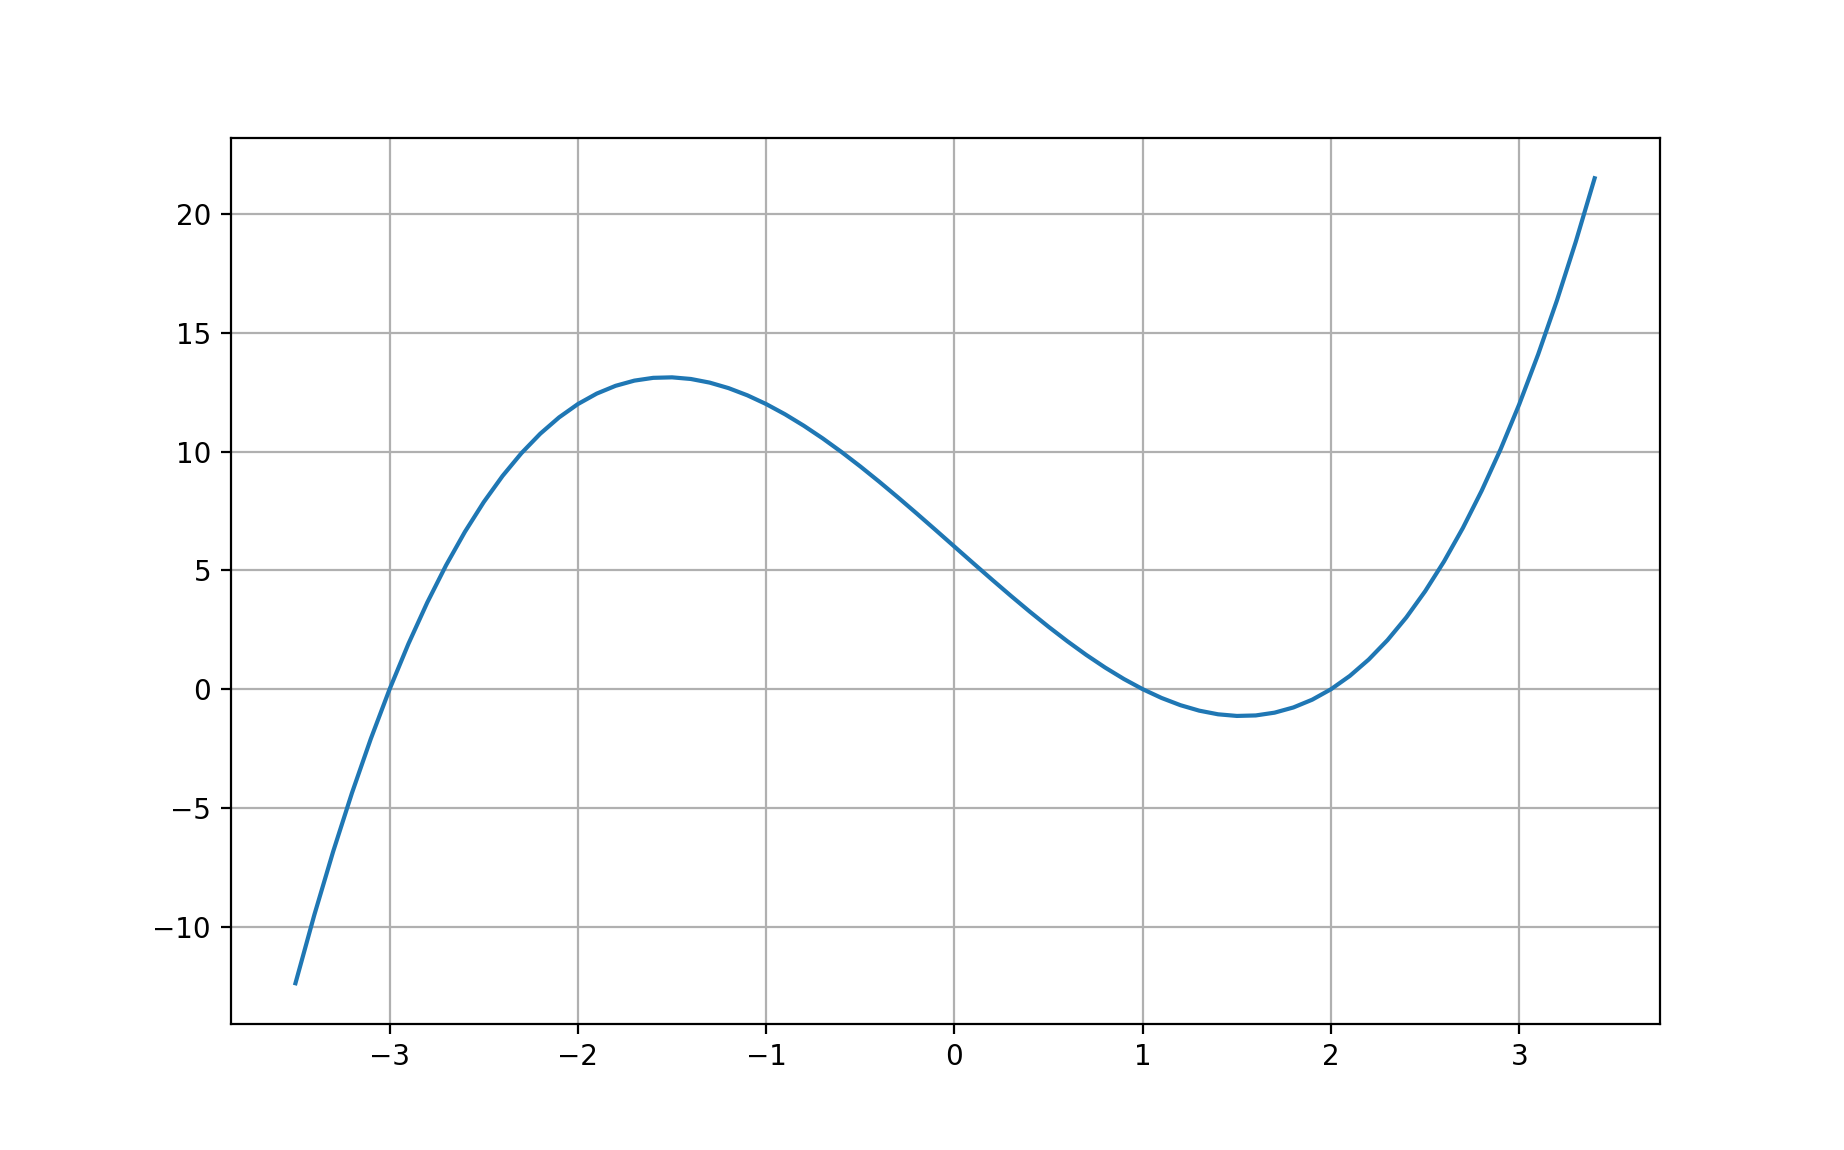
\includegraphics[width=\textwidth]{polyplot1.png}

If you received an error that the matplotlib was not found, use pip to install it:
\begin{Verbatim}[commandchars=\\\{\}]
$ \textbf{pip install matplotlib}
\end{Verbatim}

\begin{Exercise}[title={Observations}, label=plotobservations]
  Where does your polynomial cross the y-axis? Looking at the
  polynomial $x^3 - 7x + 6$, could you have guessed that value?

  \vspace{20mm}
  
  Where does your polynomial cross the x-axis? The places where a
  polynomial crosses the x-axis is called \emph{its roots}. Later in
  the course, you will learn techniques for finding the roots of a
  polynomial.
\end{Exercise}
\begin{Answer}[ref=plotobservations]
  The polynomial crosses the y-axis at 6. When x is zero, all the terms are zero except the
  last one. Thus you can easily tell that $x^3 - 7x + 6$ will cross the y-axis at $y=6$.

  Looking at the graph, you tell that the curve crosses the y-axes
  near -3, 1 and 2. If you plug those numbers into the polynomial, you
  would find that it evalutes to zero at each one. Thus, $x=-3$, $x=1$, and $x=2$ are roots.
\end{Answer}
